
% !TEX root = DesignDocument.tex

\chapter{Design  and Implementation}

\section{Systems Goals}
\begin{itemize}
	\item Provide an easy-to-use 2D simulation environment
	\item Simulate realistic physics as best as possible
	\item Support easy modification and extension of the simulation
	\item Allow saving and loading entire simulation state
	\item Allow for design of custom robots to use in the simulation
\end{itemize}

\section{System Overview and Description}
There are six major components in this system
\begin{itemize}
	\item Application core
	\item General User Interface
	\item World Visualization
	\item Physics Engine
	\item File Read/Write
	\item Plugin System
\end{itemize}
See figure \ref{fig:systemdiagram} for an overview representation of where the components reside in the application and what other components they connect to.

\begin{figure}[tbh]
\begin{center}
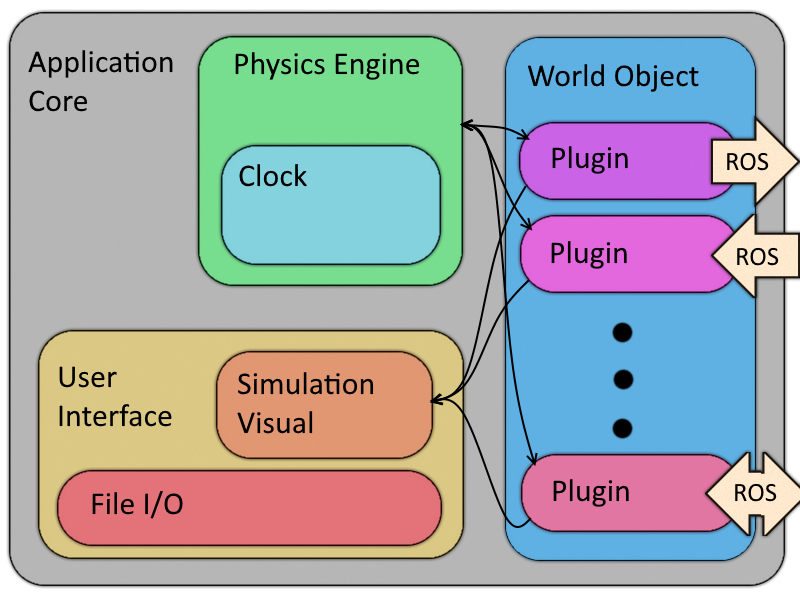
\includegraphics[width=0.75\textwidth]{./images_design/sysarch}
\end{center}
\caption{A visual representation of the system architecture, including basic data paths\label{fig:systemdiagram}}
\end{figure}

\subsection{Application Core}
The Application Core has the job of organizing the rest of the system. It connects all of the events generated by the other components and keeps track of all simulated objects. It is also responsible for adding and removing simulated objects when commanded to.

Explained in more detail below, anything simulated in the application can be represented in the World Object class. The World Object exposes functions to
\begin{itemize}
	\item Add/Remove itself from the physics engine
	\item Obtain its Models for drawing on screen
	\item Obtain its list of Properties
\end{itemize}

Models and Properties are fully defined below as well.

\subsection{Physics Engine}
The Physics Engine is the backbone of the simulation. The main purposes of the Physics Engine are
	\begin{itemize}
		\item Track what objects are part of the simulated world
		\item Step the simulated world at a regular rate
		\item Notify simulated objects when the world updates
	\end{itemize}
Forces can be applied to the simulated objects at any point in time, by any part of the application. The Physics Engine does not concern itself with where the forces originate, just the effects of them.
 
\subsection{User Interface}
The User Interface consists of all portions of the UI which are not the visualization of what is actually being simulated. The UI is responsible for things like providing the user with ways to load and save files, start and stop the simulation, and edit the properties of the simulated objects.

While the visualization of the simulated activity is, technically speaking, part of the UI, it is connected to the rest of the UI through a single interface. This allows it to be developed independently and means the rest of the UI should be agnostic to the details of how it looks and behaves. We will reference the visualization in this document with terms such as "World Visual", or "Visualization Widget".

\subsection{World Visualization}
The World Visualization is a widget in the UI which is responsible for portraying the simulated activity. Its communication is strictly with the general UI, as it is a child object of it. The UI is expected to tell this visual when objects are added and removed, as well as what models belong with those objects.

\subsection{File Read/Write}
The File Read/Write component is utilized by the general UI. When the user selects a file, the Read/Write component loads or saves a world object or collection of world objects in that file. If the file is malformed, it returns an error that the UI can display. In the future, this could be extended to support multiple different file formats.

\subsection{Plugin System}
The Plugin System keeps the core application logic separate from the specific capabilities of the simulated objects. Plugins provide the components which make up the objects simulated. Using this design allows users to write their own components for the simulation if some desired feature is missing.

\section{Technologies Overview}
\subsection{C++}
	The entire application is written using the C++ programming language. Reference material for the syntax and libraries provided as part of the language can be found at \url{http://en.cppreference.com/w/}. The most recent standard used by this project is C++11.
	
\subsection{Qt}
	Qt is a cross-platform development framework and library. It is utilized in this project for a couple of specific features it provides
	\begin{itemize}
		\item Event Loop
		\item QObjects
		\item Signals and Slots
		\item Plugins
		\item Widgets Library
		\item Graphics Framework
	\end{itemize}
	Information about the project can be found at \url{http://doc.qt.io/}. Some of the core concepts of these features are described in the following sections.
	
	An example containing QObjects and Signals and Slots can be seen in listing \ref{lst:qobjexample} below.
	
\subsubsection*{Event Loop}
	The central part of Qt is the Event Loop. When a Qt application is started, it generally enters an event loop which spins during idle time. When an event happens, it is queued until the start of the next iteration of the event loop. During each iteration of the event loop, all pending events are delivered to their receivers to be handled.
	
	\begin{lstlisting}[caption={Pseudocode for the Qt Event Loop}]
while(application_running)
{
	for(event in event_queue)
		handleEvent(event)
	Remove handled events
}
	\end{lstlisting}
	
	Many events are user-generated by actions such as clicking buttons, typing text, and resizing windows. Other events may take the form of cross-thread communication through Signals and Slots.
	
\subsubsection*{QObject}
	QObjects are the base type of anything residing in the Qt event framework. Similarly to how all Java types inherit Object, all Qt objects inherit QObject. There are two parts to QObject inheritance.
	\begin{enumerate}
		\item Inheriting QObject will add a number of common functions, signals, and slots to a type. When QObjects are instantiated, they can be given a parent QObject. When a parent QObject is destroyed, it will automatically destroy all of its children.
		\item The Q\_OBJECT macro must be placed in the \lstinline|private| portion of the class definition. At compile time, the Qt Meta Object Compiler (or MOC) is run before the standard C++ compiler. The MOC finds this macro and other Qt-specific keywords and generates standard C++ files which a normal compiler, such as g++, can use.
	\end{enumerate}
	
	Limitations on inheritance of QObject
\begin{enumerate}
	\item QObject cannot be inherited in a templated class
	\item If multiple types are inherited, QObject (or a type that isa QObject) must be the last type inherited
	\item QObject cannot be virtually inherited, so the diamond inheritance problem cannot be resolved if all types are QObjects
\end{enumerate}
	
\subsubsection*{Signals and Slots}
Signals and Slots allow programmers to define custom events and event handlers in their objects. 

A Signal is a public method of a QObject which has no definition. (The definition is added by the MOC). Instantiated QObjects can emit signals at any point in time. Signals may have parameters, and when the object emits a signal with parameters, it will fill them with data.

A Slot is a public, protected, or private method of a QObject. It must have a full definition just like any other method. (In many cases, it can be treated exactly as if it were a regular method.)

There are two main limitations on Signals and Slots
\begin{enumerate}
	\item All parameters MUST be pass-by-value. This allows all data to be copied, preventing race conditions when signals trigger slots in other threads.
	\item Custom types passed as parameters in signals and slots must be known to the Qt Meta-Object System. See documentation on the qRegisterMetaType() function for more information on how this works.
\end{enumerate}

At runtime, applications can connect the signals of instantiated QObjects to the slots of any other instantiated QObjects. When a QObject emits a signal, any slots that it is connected to will be called.


\begin{lstlisting}[language=C++, caption={Example of QObjects with parenting, Signals and Slots, and connections.\label{lst:qobjexample}}]
class foo : public QObject
{
	Q_OBJECT
public:
	//Construct with optional parent QObject
	foo(QObject* parent=nullptr) : QObject(parent){}

//Keyword known to MOC
//All signals are public methods
signals:
	void somethingHappened();
	void otherThingHappened(int);

//Another MOC keyword. Slots can be public, private, or protected
public slots:
	void reactToAnotherThing(int x)
	{
		cout << "Another thing: " << x << endl;
	}
};

class bar : public QObject
{
	Q_OBJECT
public:
	//Construct with optional parent QObject
	bar(foo* parent) : QObject(parent)
	{
		//Connect events between objects
		//Note that events and handlers have the same function signature	
		
		//When somethingHappened() is emitted by 'parent'
		//Do reactToSomething() in 'this'
		connect(parent, &foo::somethingHappened,
		        this, &bar::reactToSomething);
		
		//When otherThingHappened() is emitted by 'parent'
		//Do reactToOtherThing() in 'this'
		connect(parent, &foo::otherThingHappened,
		        this, &bar::reactToOtherThing);
		
		//When anotherThingHappened() is emitted by 'this'
		//Do reactToAnotherThing() in 'parent'
		connect(this, &bar::anotherThingHappened,
                parent, &foo::reactToAnotherThing);
	}

//Keyword known to MOC
//All signals are public methods
signals:
	void anotherThingHappened(int);	

//Another MOC keyword. Slots can be public, private, or protected
private slots:
	void reactToSomething()
	{
		cout << "Something happened!" << endl;
	}
	
	void reactToOtherThing(int x)
	{
		cout << "Reacting to other thing: " << x << endl;
		
		//Send a signal back to 'parent' object
		emit anotherThingHappened(x+1);
	}
};

int main()
{
	//Put a 'bar' on the
	foo* f = new foo();
	bar* b = new bar(f);
	
	//This will delete b as well because 
	//b is a child of f
	delete f;
}
\end{lstlisting}

\subsection{Box2D Physics}
The Box2D library is used as the basis of the Physics Engine for this simulation. It is a C++ library which can be used for realistic physics simulation and collision detection. The Box2D project is hosted on github at this location \url{https://github.com/erincatto/Box2D}.

When working with a Box2D simulation, there are a number of types that are used.
\begin{itemize}
	\item b2World: Container for everything being simulated and all extra simulation information. Bodies and Joints are added directly to the World to be simulated.
	\item b2Body: Container for physics information for one specific element of the simulation. Bodies are made up of any number of Fixtures, which are held relative to each other as the body moves. Bodies contain information such as mass, inertia, velocity, etc. Bodies can also be acted upon by forces or impulses.
	\item b2Fixture: Fixtures are used to attach shapes to a Body. Each fixture is used to attach a single shape.
	\item b2Shape: Abstract base type of any shape. Various shapes are supported by Box2D, but this project utilizes mainly b2PolygonShape and b2CircleShape.
	\item b2Joint: Joints are used to constrain how bodies move relative to each other. Many types of joints exist in Box2D, some examples are rigid, revolute, prismatic, and motor.
\end{itemize}

\subsection{ROS}
As mentioned a number of times previously, this simulation supports communication with external applications through ROS, the Robotics Operating System. Information on ROS can be found at \url{http://www.ros.org/}. The version of ROS targeted for this project is ROS Kinetic Kame.

The core application itself has minimum communication through ROS, it mainly starts a ROS listener thread so that messages can be received. The bulk of the message sending and receiving is done by the plugin components which make up the objects being simulated.

\newpage
 \section{Architecture and System Design} 	
 \subsection{Design Decisions}
  	The simulation underwent a number of design changes during its development. This section will discuss what drove the major design decisions associated with this project.
 \subsubsection*{User Experience}
	Because this application is mainly for students just being introduced to robotics and will be a tool for education, we wanted to make the simulator as user friendly as possible. We decided to try for a video game-like feel, as most individuals are familiar with video games which would make it easy to learn. 
	
	The biggest design decision we had to make for the user experience aspect of the project was whether we wanted to use a single window for everything (simulation, robot builder and map builder) or if we wanted to have multiple windows. We began with a few concepts and wire frames. 

\begin{figure}
\begin{subfigure}{0.5\textwidth}
	\begin{center}
	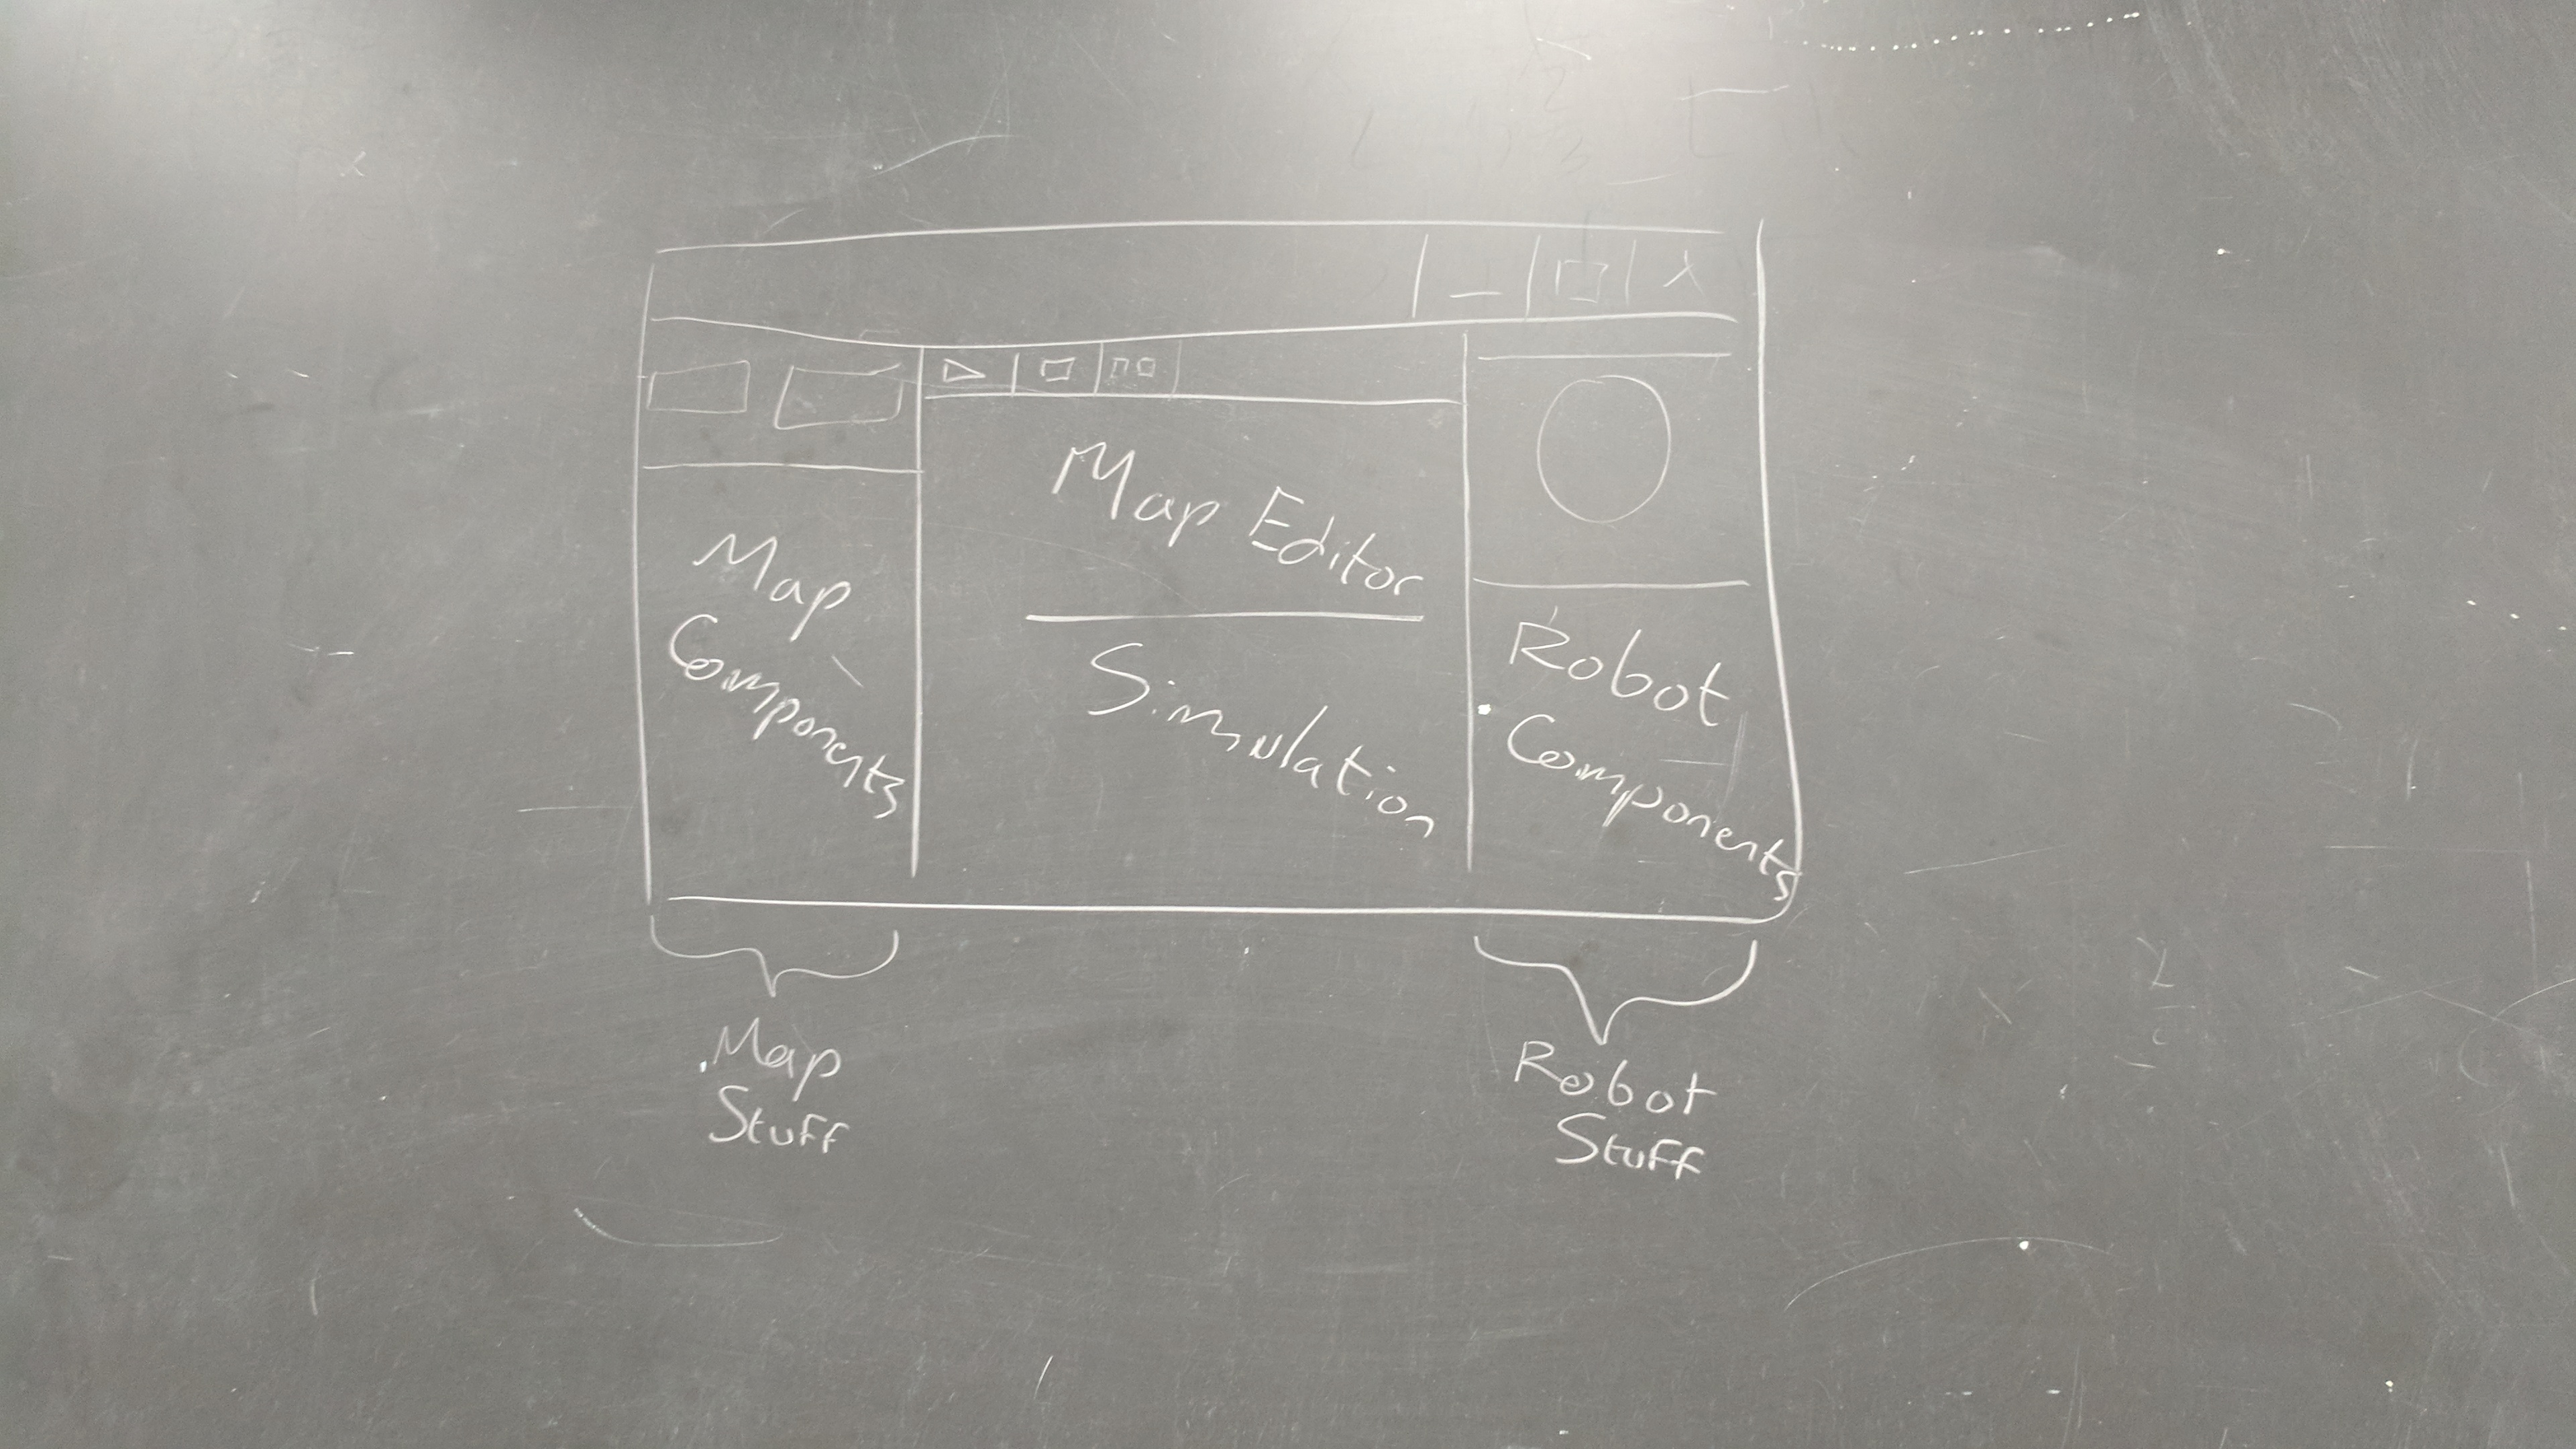
\includegraphics[width=0.9\textwidth]{./images_design/Sams.jpg}
	\caption{Single Window Concept}
	\label{fig:singlewindowconcept}
	\end{center}
\end{subfigure}
\begin{subfigure}{0.5\textwidth}
	\begin{center}
	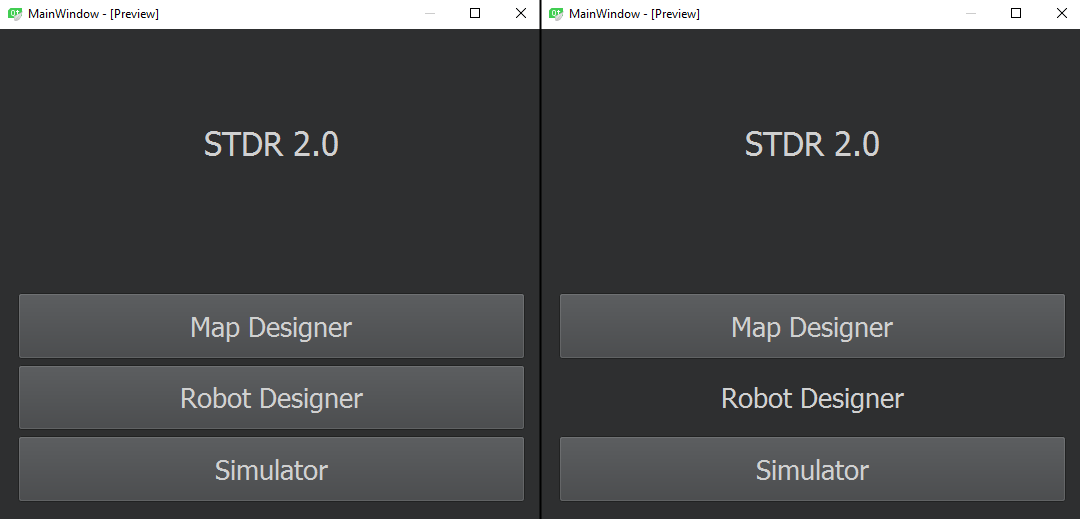
\includegraphics[width=0.9\textwidth]{./images_design/MainScreen.png}
	\caption{Multi-Window Start Window}
	\label{fig:mwindowStart}
	\end{center}
\end{subfigure}

\begin{subfigure}{0.5\textwidth}
	\begin{center}
	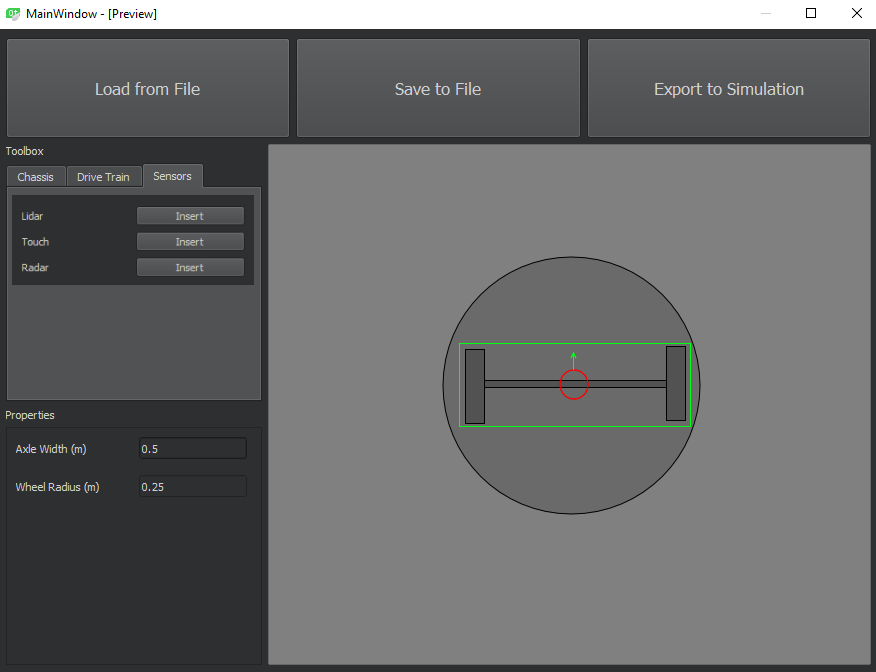
\includegraphics[width=0.9\textwidth]{./images_design/RobotDesign.png}
	\caption{Multi-Window Robot Designer}
	\label{fig:mwindowRobot}
	\end{center}
\end{subfigure}
\begin{subfigure}{0.5\textwidth}
	\begin{center}
	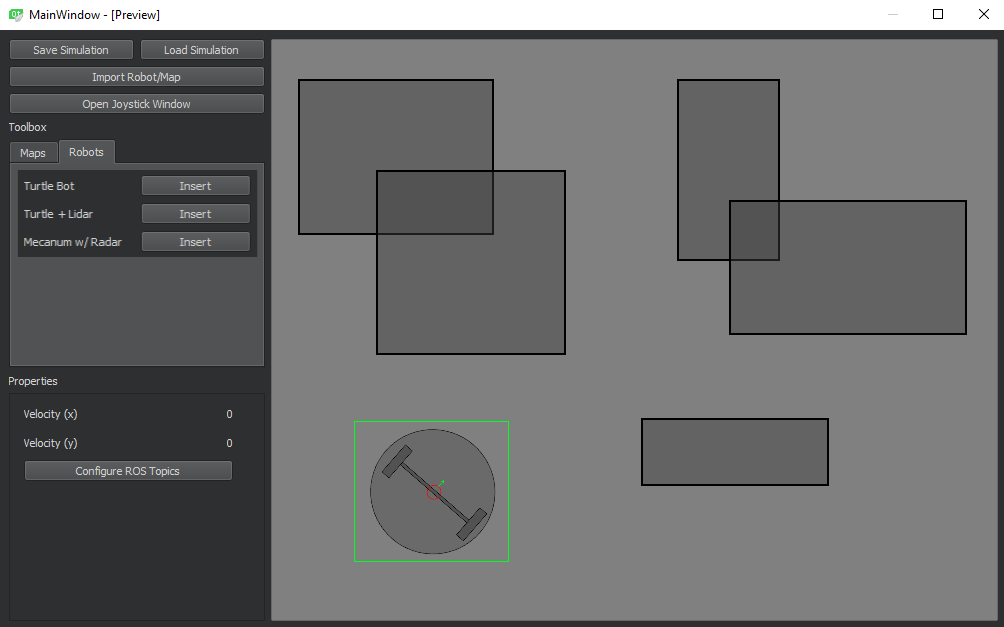
\includegraphics[width=0.9\textwidth]{./images_design/Simulation.png}
	\caption{Multi-Window Simulation}
	\label{fig:mwindowSimulation}
	\end{center}
\end{subfigure}
\caption{Example UIs presented to the Client}
\end{figure}
	
	The chalkboard drawing \ref{fig:singlewindowconcept} shows an early concept for a single window interface, while the wireframes \ref{fig:mwindowStart}, \ref{fig:mwindowRobot}, and \ref{fig:mwindowSimulation} show an idea for a multiple window interface. 

We chose to go with the single-window application both because it looks 'cleaner' and because there would be little advantage to building our application with multiple windows. It is anticipated that the user would not need to use the designer during a simulation, or the simulation during the design process; so it makes little sense to make them accessible simultaneously.  
 
 
 \subsubsection*{User Interface}
 	When building a cross-platform user interface in C++, there are only a few options available. When discussing this, the following ideas were brought up: Pure OpenGL, Qt QML, and Qt Widgets. The final decision was Qt Widgets, which will be discussed below.
 	
 	A pure OpenGL solution was not selected due mainly to the difficulty of implementation and the amount of work that would have to go into a UI of that nature. If using Qt were not an option, pure OpenGL may have been selected; however, having the Qt library available makes it hard to justify the amount of extra development that a pure OpenGL solution would add.
 	
 	When writing a UI in Qt, there are two main options for the core library: Widgets and QML. Qt Widgets has been around longer and is generally used to produce applications that look and feel 'like a desktop program'. The Widgets library contains many commonly used pieces which can be organized into a UI, similarly to how C\# Forms or Java Swing works. Qt QML is a newer library which is being actively developed with Qt. QML separates the UI entirely from the business logic by running the UI in a custom javascript interpreter. The main advantages to QML are that it's very easy to develop QML UIs without any business logic and it's currently receiving the bulk of support in new versions of Qt. QML would have been the first choice for the project UI, but it is difficult to use on a freshly installed system. Widgets projects require just a set of shared objects to run, but QML projects require a number of shared objects as well as some basic QML code files which are parsed at runtime. These additional files are not usually present in the base library installation of Qt, so using QML would have meant that the end user would need to resolve extra dependencies to run the application.
 	
 	\subsubsection*{World Visualization}
 	Within the Qt Widgets library, there are a number of different ways build a widget with a drawing canvas that shapes can be shown on. The most primitive method is to create an OpenGL drawing window which is contained in the widget. The other main option is to use the Qt Graphics Framework, which is an abstraction layer for drawing 2D objects on a background with OpenGL.
 	
 	Again, it was decided that the pure OpenGL solution would add unnecessary development time, and an alternative should be used. Not only does the graphics framework provide easy methods for drawing primitive shapes on a canvas, but it also allows for parent-child relationships between the models, which in turn allows shapes to be defined with relative transforms to each other instead of everything needing to be in world coordinates.
 	
 	\subsubsection*{Physics}
 	One of the main failings of STDR was its lack of a physics engine. It was decided early on that a known physics engine should be used, or one should be written for this project so that at least basic collision detection could be simulated.
 	
 	A number of different engines were investigated, including Box2D and Chipmunk2D. In the end, Box2D was chosen because it is simple and lightweight while also providing all of the functionality necessary for this simulator. Other physics engines would have been too bulky or difficult to use, and writing a custom physics engine would have extended the development considerably and likely would have resulted in worse performance.

	\subsubsection*{Non-Kinematic Solution}
	The original STDR operated using standard mobile robot kinematic formulas. Kinematics, and Inverse Kinematics, are systems of equations which can be used to map robot actions from control space to physical space and from physical space to control space. For example, in a kinematic solution, the robot control code may publish wheel velocities. The simulator, upon receiving these velocities, the simulator uses the forward kinematic equations of the robot to determine the overall velocity of the craft. This velocity can be used in a physics simulation.
	
	Kinematics equations of mobile robots are very specific to the driving base in use. Some commonly known ones are the Differential Drive, Mecanum Drive, and Ackermann Steer.
	The original plan for this project was to take a similar approach, using the forward kinematic formulas to produce overall craft velocities that Box2D could use. At one point, the Client mentioned that it would be cool if we didn't have to explicitly define kinematic equations for each drive system, but could let the user place wheels on a robot frame and drive it. At the time, none of the team were aware of how this could be properly simulated. The biggest issue with simulating this kind of a system is that it would be difficult to determine the proper forces to apply to keep 'no slide' conditions on a wheel. 'No slide' constraints are limitations which prevent the wheel from moving perpendicular to its intended direction of travel.
	During the implementation of the Touch Sensor Ring plugin, one team member stumbled across a tutorial outlining how to use Box2D to simulate a top-down steered vehicle that a user could drive. The tutorial showed how using different physics bodies for each wheel would allow the simulation to negate any forces which would cause the wheel to slide perpendicular to its intended direction of motion. 
	At this point, the decision was made to completely rework how robots are defined within the application. Rather than load plugins which have the kinematic equations for specific wheel bases, the user will load plugins which define how specific wheels move. Those wheels will be placed on robot frames and can apply whatever forces are necessary to constrain robot movement as they should.
	
	\subsubsection*{Single vs. Multiple Threads}
	One of the early design choices was the do as much processing in parallel as possible. It is reasonable that this project will be used to simulate large worlds with many robots, and each robot could have many sensors on it. The idea was that if all sensor calculations could be computed in parallel, the simulation would be less likely to lag behind real-time under these circumstances.
	During implementation of the Touch Sensor Ring plugin two things became evident:
	\begin{itemize}
		\item It would be more trouble than it's worth to use Box2D safely in a multithreaded application
		\item Sensor calculations will likely be fast enough that they won't impact the simulation significantly
	\end{itemize}
	After these realizations occurred, the decision was made to keep all processing in a single thread to simplify the application. The major risk to this design is that the system will lag behind real-time; however this should not affect simulations, just the observation of them. It is planned that the simulator will publish timestamp messages so that control code which relies on the passage of time can correctly account for any lag in the system.
%\section{Notable Algorithms} 
 %\subsubsection{Importing Images}

 \newpage
\subsection{Classes}
  \subsubsection*{Model}
  The Model class is a container for shapes; it is designed to be used to communicate what should be drawn on the screen. When models change or move, signals are emitted so that the image drawn can update to reflect the changes.
  
 	The UML of the Model class can be seen in UML Figure \ref{uml:model}. The Model class provides constructors to initialize it with any number of child Models and/or shapes and exposes accessor methods for both.

 \begin{figure}[h]
 	\begin{center}
 	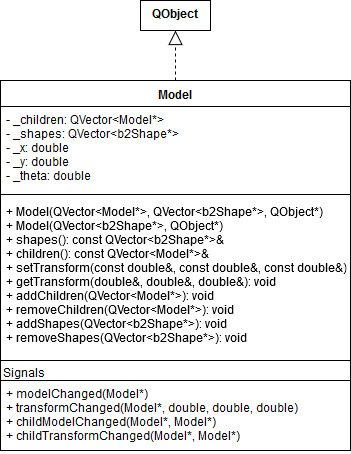
\includegraphics[scale=0.5]{./images_design/uml/Model}
 	\caption{UML of Model\label{uml:model}}
 	\end{center}
 \end{figure}  
 
 All children of a Model should exist on the heap. Upon its deletion, the Model will delete all of its children. The shapes of a Model may exist anywhere in memory, as the Model will NOT delete its shapes at any time. 
 
After construction, shapes and children models can be added and removed with the four functions
 \begin{itemize}
 	\item addChildren()
 	\item removeChildren()
 	\item addShapes()
 	\item removeShapes()
 \end{itemize} 
 
 Calling any of these functions will result in the modelChanged() signal being emitted. If a child model emits modelChanged(), then the parent will forward that call with the childModelChanged() signal. This design allows the UI to do the minimum amount of re-rendering necessary when part of a model updates.
 
 The transform of the model can be accessed through getTransform() and setTransform(). Setting the transform will result in the transformChanged() signal being emitted, and similarly to how the modelChanged() signals work, the parent of a model whose transform changes will forward that signal with childTransformChanged().
 
 Figure \ref{uml:dataflow_model} depicts the series of notifications which result from moving or modifying a Model and its child Models.
 \begin{figure}[h]
 	\begin{center}
 	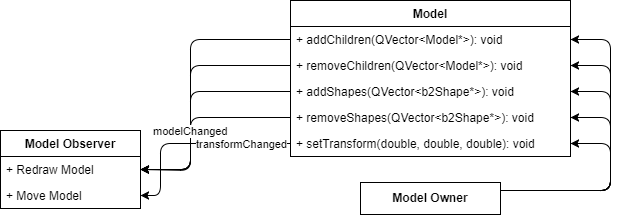
\includegraphics[width=\textwidth]{./images_design/uml/DataFlow_Model}
 	\caption{Flow of data using Models. When the Model owner updates a model: If that model is a child, it notifies its parent; if it is the parent, it notifies the observer.\label{uml:dataflow_model}}
 	\end{center}
 \end{figure}   
 
 \subsubsection*{Property}
 	Properties are variables within an object that may be modified by external sources. They are accessed through PropertyView objects, which enforce read/write rules so that internal state that should not be changed is not changed by accident. The UML Diagrams for Properties, PropertyViews, and all associated types are found in Figure \ref{uml:property}
 	
 \begin{figure}[h!]
 	\begin{center}
 	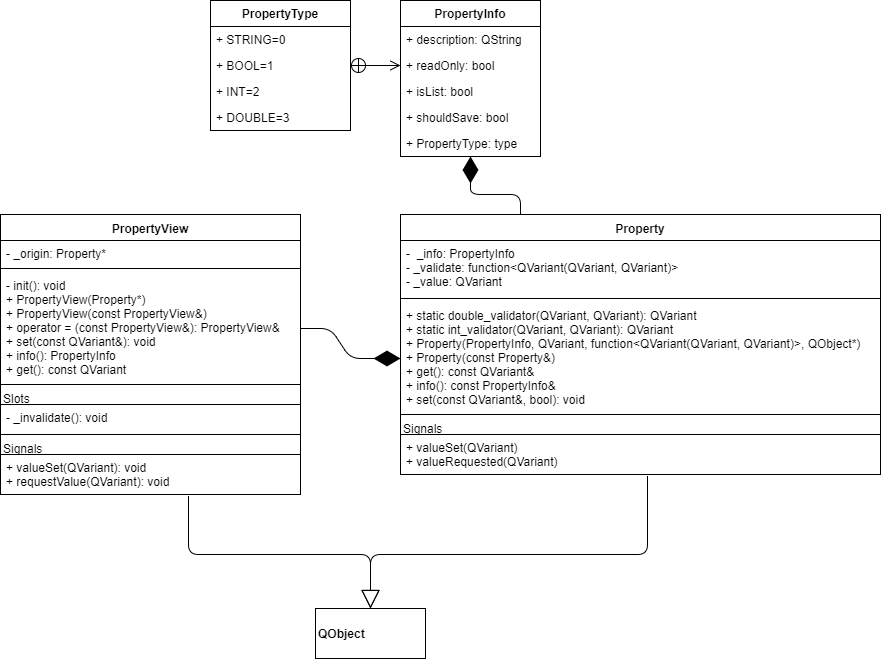
\includegraphics[width=\textwidth]{./images_design/uml/Property}
 	\caption{UML of Property and associated classes\label{uml:property}}
 	\end{center}
 \end{figure} 
 
 	A Property has three main parts
 	\begin{itemize}
 		\item Its PropertyInfo
 		\item A validation function
 		\item Its value
 	\end{itemize}
 	
 	The PropertyInfo is a container for any meta information about the Property. This contains data such as the type of the data, whether or not it's read-only, whether or not it's a list, and a description of what the Property is used for. This is intended to be used to aid a UI which displays Properties to the user. It is assigned to a Property once, at construction, and can be accessed through the info() method.
 	
 	The validation function follows the prototype \lstinline|function<QVariant(QVariant, QVariant)>| and is used to make sure that the data assigned to the Property is valid. The first parameter represents the previous value, and the second parameter is a potential new value. The function should return the new value if it is acceptable and the old value if the new one is not acceptable (Optionally, the function may change the new value to make it valid and then return it). The default validation function accepts all values. A number of basic validation functions exist as static methods of the Property class for convenience. Some of them are
 	\begin{itemize}
 		\item double\_validator()
 		\item int\_validator()
 	\end{itemize}
 	
 	The value of a property is accessed and mutated though the methods set() and get(). get() returns the current value. set() validates a new value using the validation function and stores whatever value is returned. Whenever the set() function is called, the valueSet() signal is emitted with the value that was set. This happens even if the stored value does not change.
 	
 	The PropertyView object contains all of the same public functions as a Property; however it is constructed with only a Property, which it observes. When the set() function is called on a PropertyView, the requestValue() signal is emitted, and the original Property handles that signal and validates the new value. The valueSet() signal in a PropertyView is tied to the same signal in its observed property so that any owner of a PropertyView will know when the value changes.
 	
 	The internal slot \_invalidate() is called when the observed Property is destroyed to prevent a null reference. If any accessors are called after this happens, they will return default-constructed values. It is intended that the owner of a PropertyView will receive some indication that the PropertyView should no longer be tracked from another source.
 	
 	Figure \ref{uml:dataflow_property} shows the flow of data between properties, property owners, property views, and property observers.
 	
 \begin{figure}[h]
 	\begin{center}
 	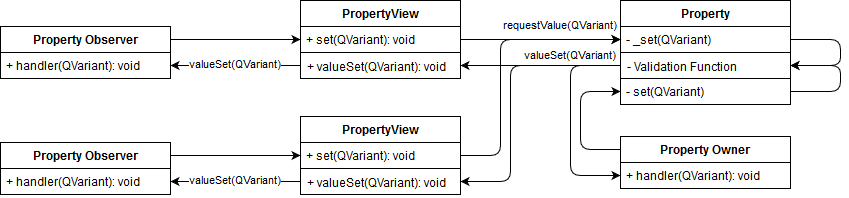
\includegraphics[scale=0.5]{./images_design/uml/DataFlow_Property}
 	\caption{Data flow of Properties, their owners, and their observers. Note that any time a value is set (Either through a PropertyView or directly) the data is validated before the new value is sent to the owner and any observers.\label{uml:dataflow_property}}
 	\end{center}
 \end{figure} 
 	
  \subsubsection*{World Object} \label{sec:worldobjclass}
	The main data type in this simulation is the World Object. World Objects can be added to and removed from the simulation, cloned, and saved to or loaded from files. World Objects consist of a set of Components (Which follow the WorldObjectComponent\_If interface and are created by plugins) and the constraints that keep them together. For the UML diagram of a World Object, see Figure \ref{uml:worldobj}.
	
 \begin{figure}[h]
 	\begin{center}
 	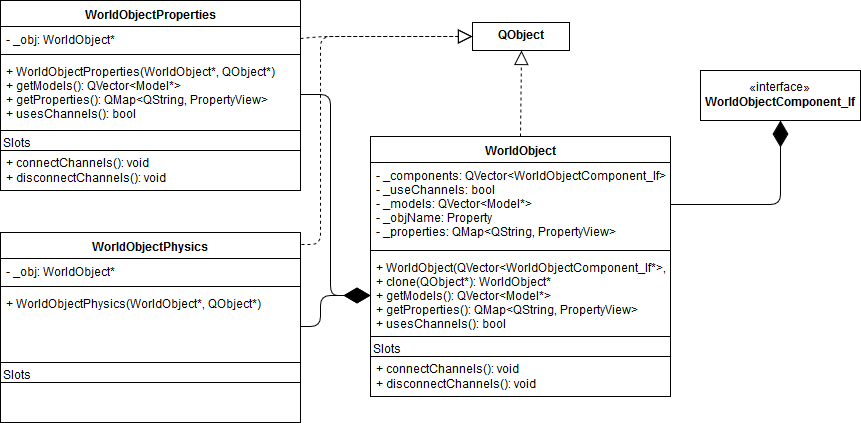
\includegraphics[scale=0.5]{./images_design/uml/WorldObj}
 	\caption{UML of World Object and associated classes\label{uml:worldobj}}
 	\end{center}
 \end{figure}
 \hrule	
	TODO
	\begin{enumerate}
		\item Finalize new iteractions between World Object and Physics Engine
	\end{enumerate}
\hrule
	World Objects, upon construction, consolidate all of the models and properties of their components. When getModels() or getProperties() is used to access the World Object, these consolidated lists are returned.
	
	It is possible that some of a World Object's components will use external communications, such as ROS. The usesChannels() accessor is used to determine if this is the case, and the connectChannels() and disconnectChannels() slots are used to start or stop communctions of any components which do this.
	
	Only the Simulator Core holds the reference to a World Object in the simulation. As can be seen in the UML diagram, a number of wrapper objects exist to provide specific interfaces. The WorldObjectProperties class provides an interface to a World Object which is used by the User Interface, and the WorldObjectPhysics provides the interface used by the Physics Engine. These interfaces are children (in the Qt sense) of the original World Object, so no owner of an interface needs to delete their interface when the WorldObject is removed from the simulation.
	
	When a World Object is added to the physics engine, it should be given access to the Box2D world. At this point, the World Object and its Components create any Box2D bodies needed and set up the shapes, masses, and joints required to simulate the World Object. During the simulation, Components can apply forces to this body to give motion to the World Object. When the World Object is removed from the physics engine it should be given access to the Box2D world again so that all bodies and joints can be removed from the simulation. These two events are the only points in time that the World Object will add or remove elements of the simulated world.
  
  
  \subsection{Interfaces}
  \subsubsection*{Physics Engine Interface}
  The SimulationPhysics\_If interface (UML Figure \ref{uml:phys_if}) provides the interface any Physics Engine used in this simulation must follow. It is expected that any Physics Engine will be built on Box2D.
  
 \begin{figure}[h]
 	\begin{center}
 	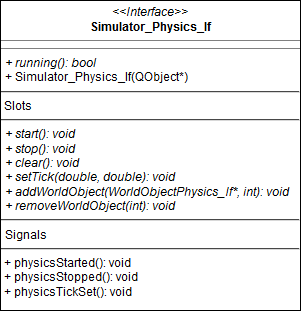
\includegraphics[scale=0.5]{./images_design/uml/Physics_Engine_If}
 	\caption{UML of Physics Engine class interface\label{uml:phys_if}}
 	\end{center}
 \end{figure}  
  
  There are four main methods for modifying the flow of the simulation and two main methods for influencing what is actually simulated.
  
  The methods for changing simulation flow are
  \begin{itemize}
  	\item start()
  	\item stop()
  	\item clear()
  	\item setTick()
  \end{itemize}
  
  The methods for adding and removing simulated objects are
  \begin{itemize}
  	\item addWorldObject()
  	\item removeWorldObject()
  \end{itemize}
  
  The Physics Engine should emit the following signals under appropriate circumstances.
  \begin{itemize}
  	\item physicsStarted()
  	\item physicsStopped()
  	\item physicsTickSet()
  \end{itemize}
  
  \subsubsection*{UI Interface}
  A UI for this simulation is expected to provide users with the following features
  \begin{itemize}
  	\item Add/Remove elements from the simulation
  	\item Start/Stop/Time Warp the simulation
  	\item Display Error messages
  \end{itemize}
  
  The UML diagram of this interface (Figure \ref{uml:ui_if}) defines the exact signals and slots that are expected for these functions.
 \begin{figure}[h]
 	\begin{center}
 	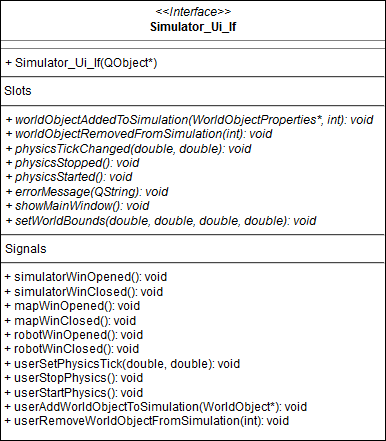
\includegraphics[scale=0.5]{./images_design/uml/Ui_If}
 	\caption{UML of UI class interface\label{uml:ui_if}}
 	\end{center}
 \end{figure}
 
 All data flow with the UI should follow a circular pattern. This means that, when the UI generates a signal, it should not update until a response has been received. This prevents the UI from getting out of sync with the rest of the application. This is the explanation for each signal having a corresponding slot. The UI should emit the signal and only update the screen when the slot is called.
 	
  \subsubsection*{View Widget Interface}
  The View Widget interface is a requirement of the specific UI written for this project. It provides a standardized way for the MainWindow UI class to update the world view widget, regardless of what drawing library that widget uses.
  
  This interface provides methods which allow
  \begin{itemize}
  	\item Setting the size of the world
  	\item Adding and removing models associated with an object
  	\item Changing how models for an object are drawn
  	\item Selecting objects and indicating selection
  \end{itemize}
  
  As with the general UI interface, the Visual Widget should not update the selected object when the user click event happens, but instead should signal that the user selected an object and wait for the objectSelected() method call.
 \begin{figure}[h]
 	\begin{center}
 	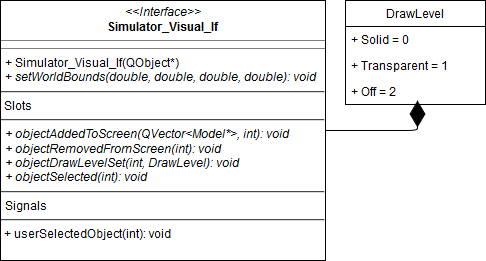
\includegraphics[scale=0.5]{./images_design/uml/Visual_If}
 	\caption{UML of Visualization widget interface\label{uml:visual_if}}
 	\end{center}
 \end{figure}
  \subsubsection*{File Handler Interface}
  Like the View Widget Interface, this interface is a requirement of the UI implemented for this project. One of the goals of the application is to be able to load and save robots, maps, and simulations. Because all of these things are represented as a World Object or collection of World Objects, a single file interface is needed. The File I/O object should be able to load and save files with 1-n world objects contained in them.
   \begin{figure}
 	\begin{center}
 	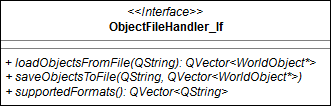
\includegraphics[scale=0.5]{./images_design/uml/FileHandler_If}
 	\caption{UML of File Handler interface\label{uml:filehandle_if}}
 	\end{center}
 \end{figure}
  \subsubsection*{World Object Component Interface}
  World Object Components are, as described above, the pieces which make up World Objects. It is expected that all components will come from plugins which are loaded by the application at runtime. This provides flexibility for users, as it will allow them to define their own robot sensors and wheels as well as map obstacles.
 \begin{figure}
 	\begin{center}
 	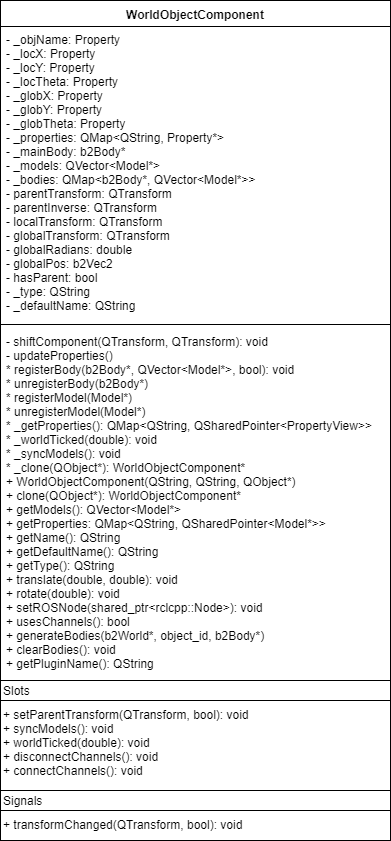
\includegraphics[scale=0.5]{./images_design/uml/WorldComponent_If}
 	\caption{UML of World Component class interface\label{uml:worldcomponent_if}}
 	\end{center}
 \end{figure} 
 World Object Components are also the application's main points of contact to the outside world. Components may register as many publish and subscribe channels in ROS as they need. At any point, they need to be able to stop listening (disconnectChannels()) or start listening(connectChannels()) on these topics. If the component does not use any channels, it should return \textit{false} in the usesChannels() method so that the system knows that these calls are unnecessary for this component.
 \hrule
 TODO
 \begin{enumerate}
 	\item Determine how World Object Components access the physics engine (See World Object TODO)
 \end{enumerate}
 \hrule
  \subsubsection*{World Object Component Plugin Interface}
  This interface defines how plugins containing World Object Components should look. Plugins are loaded using the Qt Plugin Loader; information on the plugin system can be found at \href{http://doc.qt.io/qt-5/plugins-howto.html#the-low-level-api-extending-qt-applications}{http://doc.qt.io/qt-5/plugins-howto.html}. 
  The only purpose of these plugins is to create instances of the World Object Component they contain. These instances will be cloned or added into World Objects.
 \begin{figure}[h]
 	\begin{center}
 	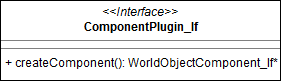
\includegraphics[scale=0.5]{./images_design/uml/ComponentPlugin}
 	\caption{UML of Plugin interface\label{uml:componentplugin}}
 	\end{center}
 \end{figure} 
 
 \subsection{Data Flow}
 All data flows between the major system components through Qt Signals and Slots. There are four main events which drive data flow
 \begin{itemize}
 	\item World Object Added
 	\item World Object Removed
 	\item Simulation Ticked
 	\item Plugin Receives External Input
 \end{itemize}
 
 \subsubsection*{World Object Added}
 	World Object additions are generally initiated by the UI. When the user wants to add an Object to the simulation, the UI signals to the core indicating what Object should be added. The core copies the World Object and stores the copy with an index. The Object and its index are sent back to the UI and Physics engine wrapped in interfaces which can be used to access methods of the new World Object.
 	
 	\begin{figure}[h]
 		\centering
 		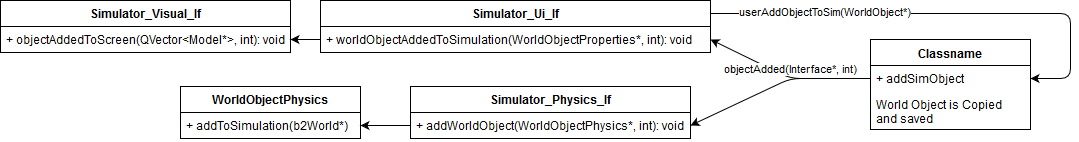
\includegraphics[width=\textwidth]{./images_design/uml/event_addObject}
 		\caption{Data flow when a new object is added to the simulation\label{uml:addevent}}
 	\end{figure}
 	
 	When the Physics engine receives a new World Object, it passes the b2World object
of the simulation to it so that the Object can add bodies and shapes to the physics engine.

	When the UI receives a new World Object, it passes the object's Model to the world view to be drawn and caches the list of object Properties. When the user selects this Object, those Properties are displayed for viewing and editing.
	
 \subsubsection*{World Object Removed}
 The process of removing a World Object is very similar to that of creating one. The UI signals to the core that the user would like to remove an Object; this Object is identified by the index that was assigned when it was added to the simulation. The core then signals back to the UI and Physics that this Object is removed and deletes the associated Object from the heap.
 
 	\begin{figure}[h]
 		\centering
 		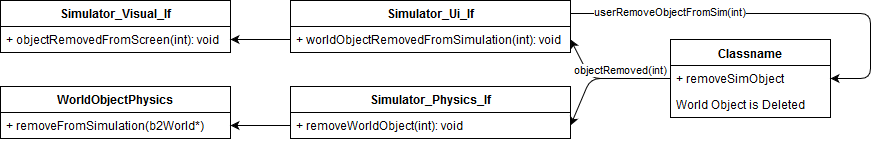
\includegraphics[width=\textwidth]{./images_design/uml/event_removeObject}
 		\caption{Data flow when an object is removed from the simulation\label{uml:removeevent}}
 	\end{figure} 
 
 When the Physics engine receives this signal, it passes the b2World to the Object again so that the Object can remove any Box2D bodies and joints that it created.
 
 When the UI receives this signal, it un-caches the Object's list of Properties and notifies the world view widget to stop drawing the Models associated with the object.
 
 \subsubsection*{World Ticked}
 World ticks are generated by the physics engine on a timer. The default tick rate is 100 per second, and each tick moves the simulation forward $\frac{1}{100}$ of a second.
 
 When a Component of an Object receives this signal, it may update its own Model, which would redraw the screen with the change. Additionally, Components can take this moment to modify the simulation by applying forces on their Box2D bodies or send messages to external applications through ROS.
 
  	\begin{figure}[h]
 		\centering
 		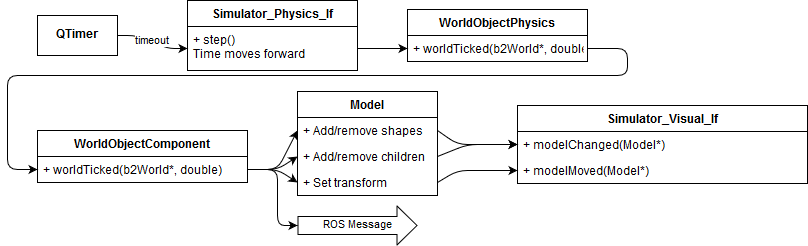
\includegraphics[width=\textwidth]{./images_design/uml/event_tick}
 		\caption{Data flow of a simulation tick\label{uml:tickevent}}
 	\end{figure}
 
 \subsubsection*{External Communication}
 The most common example of external communication is robot control code signaling that wheel velocities should change. When World Object Components receive an external communication of this nature, they can apply forces on their associated Box2D body to affect the simulation and update their models. This change will be applied on the next tick to happen after the force is applied.
 
  	\begin{figure}[h]
 		\centering
 		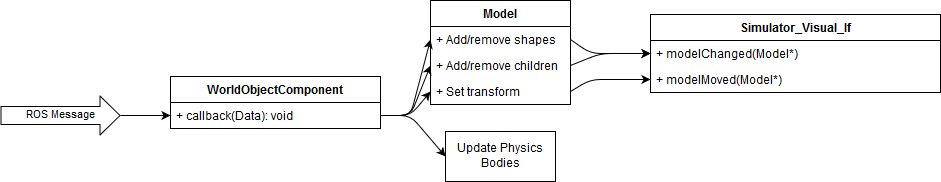
\includegraphics[width=\textwidth]{./images_design/uml/event_data}
 		\caption{Data flow of a ROS message being received\label{uml:dataevent}}
 	\end{figure}
 
\subsection{Simulator Core}

\subsubsection*{Technologies Used}
\begin{itemize}
	\item Qt
\end{itemize}

\subsubsection*{Overview}
The simulator core is, as the name suggests, the main piece of the simulation. It organizes the other parts of the system and ensures that data flows in the correct paths. The main purpose of the simulator core is to connect the UI to the Physics engine and keep them synchronized so that what's shown on screen reflects what's simulated in the physics engine. See UML Figure \ref{uml:simcore} for a list of data members and functions in the simulator core. The specific data connections set up by the core are shown in Figure \ref{uml:dataflow_simcore}.

 
 \begin{figure}[h]
 	\begin{center}
 	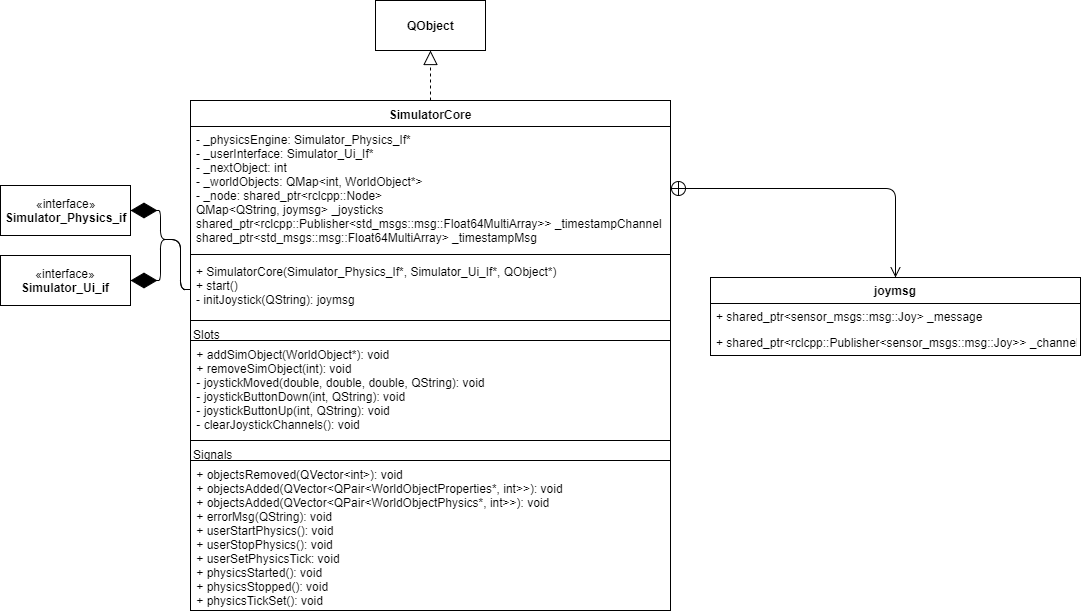
\includegraphics[scale=0.5]{./images_design/uml/SimCore}
 	\caption{UML of Simulator Core\label{uml:simcore}}
 	\end{center}
 \end{figure}

 \begin{figure}[h]
 	\begin{center}
 	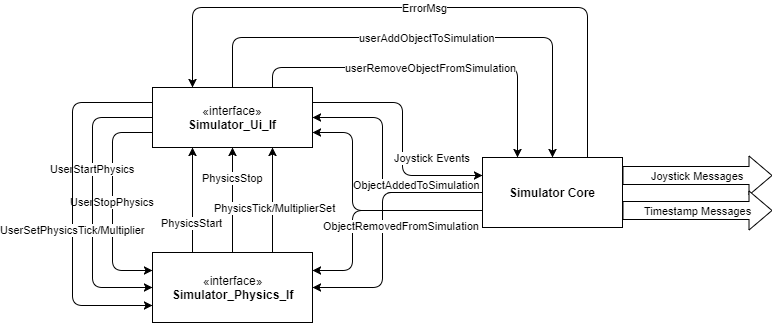
\includegraphics[scale=0.5]{./images_design/uml/DataFlow_simcore}
 	\caption{Data connections created by the Simulator Core\label{uml:dataflow_simcore}}
 	\end{center}
 \end{figure} 

\subsubsection*{Design Details}
\begin{itemize}
	\item World Objects are assigned an unsigned index when they are added. These indexes count up from 1. 0 can safely be used elsewhere as a placeholder for None.
	\item Added World Objects are cloned, so the original copy must be deleted correctly wherever it exists.
	\item The Simulator\_Ui\_If* and Simulator\_Physics\_If* that are used to construct the core will be deleted by the core's destructor.
\end{itemize}

\subsection{Physics Engine}

\subsubsection*{Technologies  Used}
\begin{itemize}
	\item Qt
	\item Box2D
\end{itemize}

\subsubsection*{Component  Overview}
The physics engine is responsible for updating the world state at regular intervals. When objects are first added to the world, they should be initialized in the physics engine, and until they are removed from the world they should be simulated along with the rest of the objects. The physics engine should be capable of starting, stopping, changing rate, and adding or removing an object while in any state. The current physics engine is the 'BasicPhysics' object found in UML Figure \ref{uml:physics}. The interface that it follows is found in UML Figure \ref{uml:phys_if}

 \begin{figure}[h]
 	\begin{center}
 	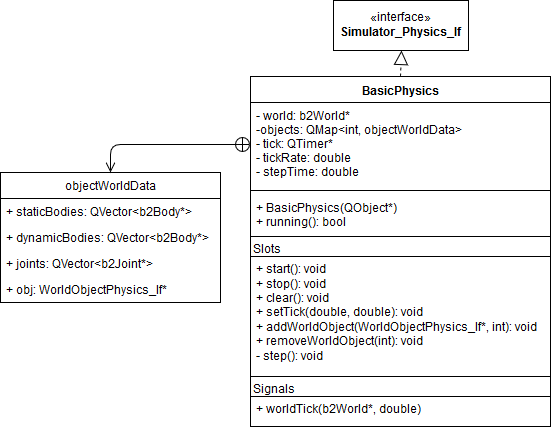
\includegraphics[scale=0.5]{./images_design/uml/BasicPhysics}
 	\caption{UML of Physics Engine\label{uml:physics}}
 	\end{center}
 \end{figure}

 \begin{figure}
 	\begin{center}
 	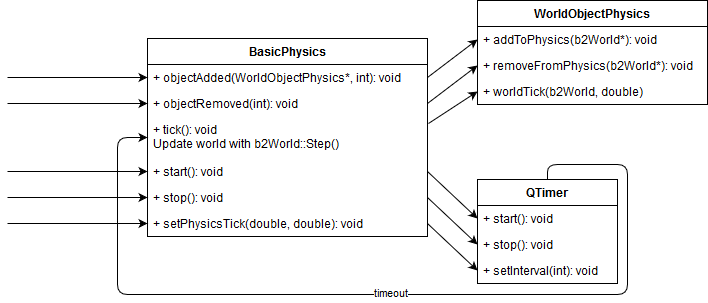
\includegraphics[scale=0.5]{./images_design/uml/DataFlow_physics}
 	\caption{Data Flow in Physics Engine\label{uml:dataflow_physics}}
 	\end{center}
 \end{figure}

\subsubsection*{Design Details}
\begin{itemize}
	\item Two things happen on every tick: The world updates (b2World::Step), then all world objects are notified of the tick
	\item The QTimer is started and stopped with QTimer::start, QTimer::stop. This means that if processing a tick takes longer than the set interval, the timer events will start to stack up. It may be necessary to look at a different method of ticking to prevent this.
\end{itemize}

\subsection{User Interface}
\subsubsection*{Technologies Used}
\begin{itemize}
	\item Qt
	\item Qt Widgets
\end{itemize}
\subsubsection*{Overview}
The user interface implemented for this project has the following features
\begin{itemize}
	\item Start/Stop simulation
	\item Time Warp simulation
	\item Add/Remove simulated item
	\item Load/Save simulation states
	\item Save a screenshot of the simulation
\end{itemize}

\hrule
TODO
\begin{itemize}
	\item Design mode - design, build, document, and test
	\item Time Warp
	\item Resetting
	\item Saving/Loading full simulations
	\item Loading Image files
\end{itemize}
\hrule

 \begin{figure}
 	\begin{center}
 	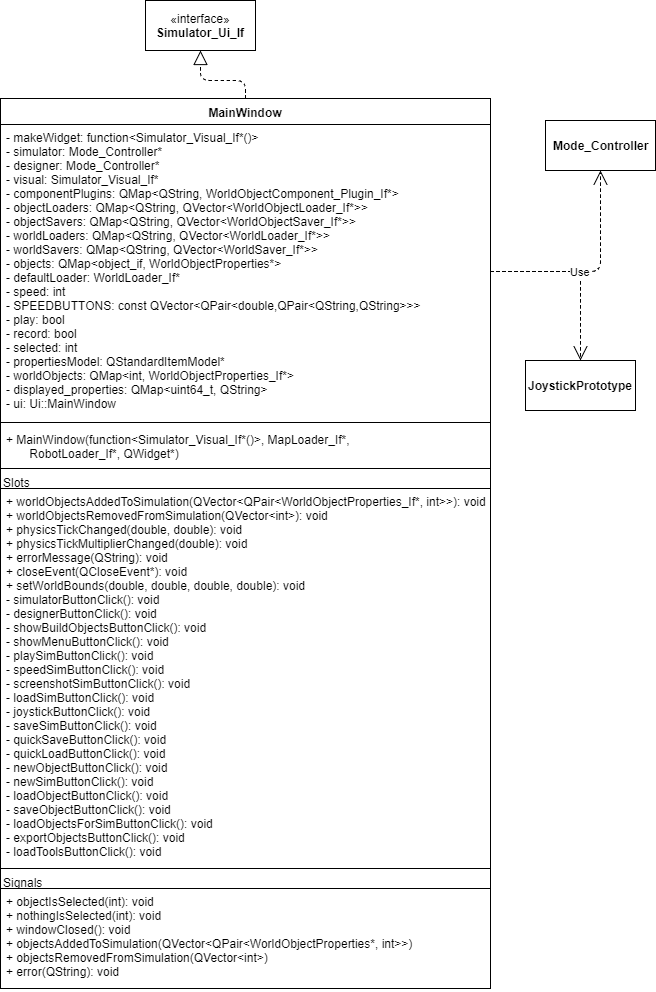
\includegraphics[scale=0.5]{./images_design/uml/MainWindow}
 	\caption{UML of User Interface\label{uml:mainwin}}
 	\end{center}
 \end{figure}
 
 \begin{figure}
 	\begin{center}
 	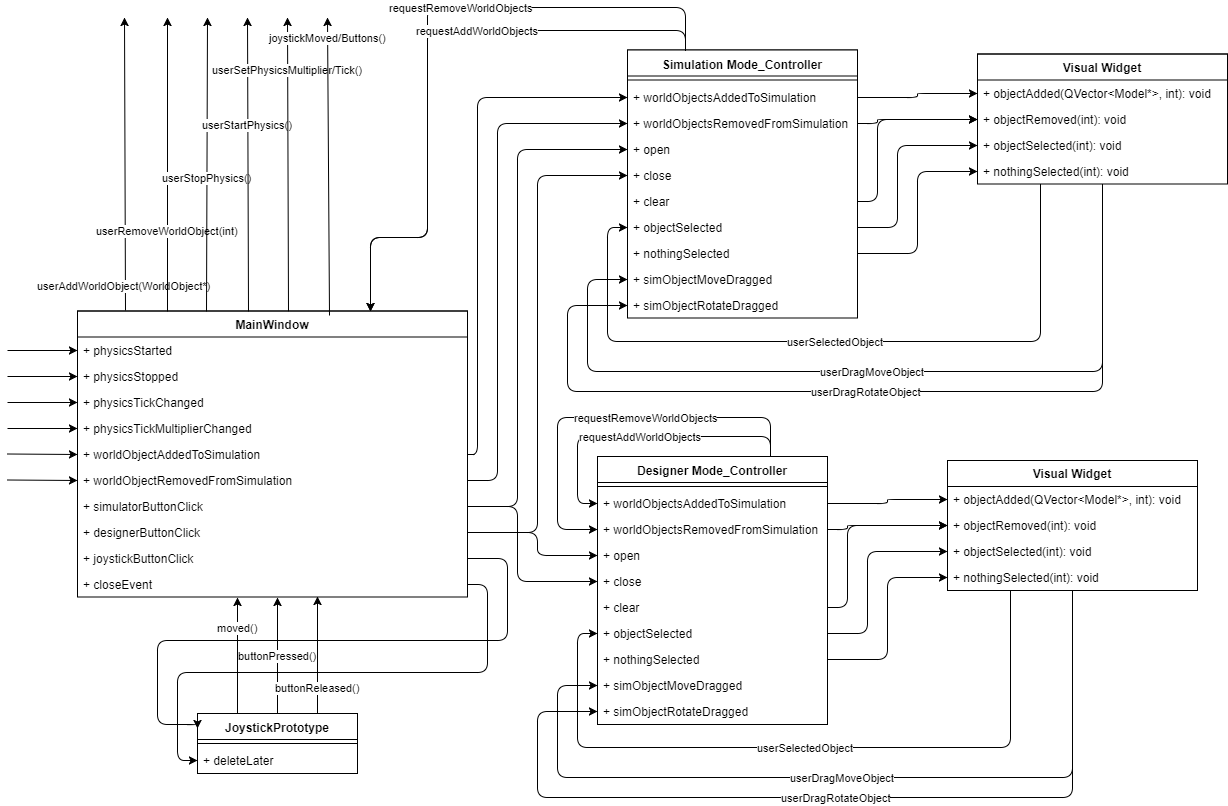
\includegraphics[scale=0.5]{./images_design/uml/DataFlow_UI}
 	\caption{Data flow of User Interface\label{uml:dataflow_ui}}
 	\end{center}
 \end{figure} 
 
 \subsubsection*{Layout}
  \begin{figure}[h!]
 	\begin{center}
 	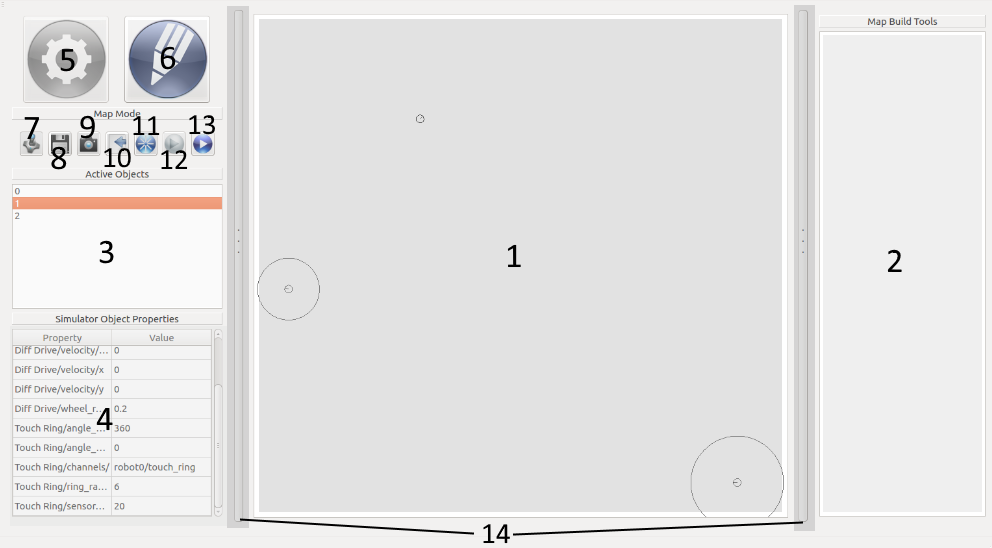
\includegraphics[width=\textwidth]{./images_design/UI_Overview}
 	\caption{Layout of the User Interface\label{fig:ui_overview}}
 	\end{center}
 \end{figure}
 
 Brief descriptions of the sections of the UI (Figure \ref{fig:ui_overview}).
 \begin{enumerate}
 	\item The World View widget\\
 	In Simulation Mode: Shows what's currently happening in the simulation\\
 	In Design Mode: Shows the world object that's currently being designed.
 	\item The toolbox\\
 	In Simulation Mode: Lists World Objects that have been loaded from file. They can be dragged into the simulation when it is not running.\\
 	In Design Mode: Shows the World Object Components which can be added to the World Object
 	\item Objects list\\
 	In Simulation Mode: Lists all World Objects currently in the simulation. They can be selected from this list.\\
 	In Design Mode: Lists all World Object Components currently on the World Object. They can also be selected from here.
 	\item Properties list\\
 	Both Modes: Displays and allows editing of whatever is currently selected
 	\item Simulation Mode button
 	\item Design Mode button
 	\item Opens a new joystick window
 	\item Saves the current simulation state
 	\item Takes a screenshot of the simulation
 	\item Opens a simulation, image (map), or world object file.
 	\item Time Warp
 	\item Resets the simulation
 	\item Starts/Pauses the simulation
 \end{enumerate}
 
 \subsubsection*{Design Details}
 \begin{itemize}
 	\item All events that affect the simulation backend (the physics or core) follow a circular data path. The UI generates an event and emits it $\rightarrow$ The affected object receives the event, acts on it, and sends a response $\rightarrow$ The UI receives that response and updates so the user knows what happened.
 	\item Object properties are shown through a Model-View controller. When an object is selected, its properties are loaded into the model and connected to the dataChanged signals it emits. When the user changes the data in the model, the property views read the new data and attempt to set it on the original Property object if the property is read-only.
 	\item The UI is constructed with a factory function for making the world view widget. This can be done because the widget follows a specific interface and allows for rewriting the world view without changing any of the rest of the application.
 	\item BUG: Currently, the user can change a read-only property on screen (this does not change the original property value, but the screen shows incorrect data)
 \end{itemize}
\subsection{World View}
\subsubsection*{Technologies Used}
\begin{itemize}
	\item Qt
	\item Qt Widgets
	\item Qt Graphics Framework
	\item Box2D
\end{itemize}
\subsubsection*{Overview}
The world viewer widget implemented in this project is called 'BasicViewer'. It uses the Qt Graphics Framework to create a 2D drawing canvas. The UML diagram for this class can be see in Figure \ref{uml:viewwidget}.

The UI can draw things on the widget by passing it a set of Models along with an integer reference. This reference could be the identifier of a World Object which the models represent, or it could be assigned by the UI. When the UI wants to change how this set of models is drawn, or remove them from the screen, this identifying value is used.
The options for how a shape is drawn include 'selected' or 'not selected', and 'solid', 'transparent', and 'not drawn'. Only one object (group of shapes with a single identifier) may be selected at a time.
 \begin{figure}
 	\begin{center}
 	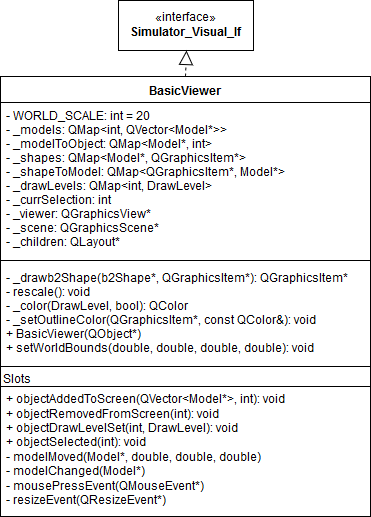
\includegraphics[scale=0.5]{./images_design/uml/BasicViewer}
 	\caption{UML of Visualization widget\label{uml:viewwidget}}
 	\end{center}
 \end{figure}
 
\subsubsection*{Design Details}
\begin{itemize}
	\item The viewer supports drawing any Box2D Shape type except for the b2ChainShape. 
	\item The widget contains both the QGraphicsScene and QGraphicsView internally. It lays out the QGraphicsView to fill itself completely on instantiation.
	\item The QGraphicsView::fitInView method appears to be broken in Qt 5.5, so the BasicView widget manually sets the viewport when it resizes.
	\item Rather than redraw an entire model when one of its children changes or moves, the widget connects to the signals of all the child models and just redraws the portions that change or move

\subsection{The main() Function}
\subsubsection*{Technologies Used}
\begin{itemize}
	\item Qt
	\item ROS
\end{itemize}

\subsubsection*{Overview}
The main() function serves a couple of important purposes.
\begin{enumerate}
	\item Create QApplication. This runs the event loop and represents the application as a whole.
	\item Call ros::spin() in a separate thread
	\item Connect the ros spin thread to the QApplication
	\item Load all valid plugins that can be found in \lstinline|../|
	\item Instantiate a system object for each interface
	\begin{itemize}
		\item ObjectFileHandler\_If
		\item Factory function for Simulator\_Visual\_If
		\item Simulator\_Physics\_If
		\item Simulator\_Ui\_If
	\end{itemize}
	\item Instantiate and start the Simulator Core
	\item Start the Qt Event Loop
\end{enumerate}

\subsubsection*{Design Details}
\begin{itemize}
	\item The ROS spin thread is connected to the QApplication for mutually assured destruction. If the ROS connection dies, then the application will close. If the Application closes, then the ROS connection will end. This prevents either from continuing in an invalid state without the other.
	\begin{lstlisting}
QFutureWatcher<void> rosThread;
rosThread.setFuture(QtConcurrent::run(&ros::spin));
QObject::connect(&rosThread, &QFutureWatcher<void>::finished, &app,
                 &QCoreApplication::quit);
QObject::connect(&app, &QCoreApplication::aboutToQuit,
                 [](){ros::shutdown();});
	\end{lstlisting}
	\item The directory above the executable is checked for plugins because that is, by default, where Catkin places shared libraries
\end{itemize}
\section{Plugins}
One of the main advantages to the design of this project is that it can be extended through WorldObjectComponent Plugins. Unfortunately, because it is a ROS package, the project (and any such plugins) must be built with Catkin and CMake. A number of plugins have been included with the project to provide much basic functionality, and those plugins can be used as examples of how plugins should be set up; however, not all plugins will follow the same patterns, so this section will describe the existing plugins as well as some of the requirements to build and use a plugin.
\subsection{Touch Sensor Ring}
The touch sensor ring plugin mimics a ring of touch sensors with a specific radius. It is intended to be used on circular robots, so that its radius can be set to the same as the robot. 
	The sensor ring can be set to sense a specific section of the circle, and the number of sensors used can be specified. Whenever the state of one of the buttons changes, a ROS message is published. Extra circles are drawn on the world visualization to show which touch sensors are triggered. An example of this can be seen in Figure \ref{fig:touchsensorexample}. Details of the properties exposed by the plugin and the ROS messages it utilizes can be found in tables \ref{tab:touch_ring_props} and \ref{tab:touch_ring_msgs}
	
	\begin{figure}[h]
		\centering
		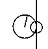
\includegraphics{./images_design/touch_sensor}
		\caption{Example of the touch sensor ring sensing something. The large circle is a robot, the small circle is the touched sensor point.}
		\label{fig:touchsensorexample}
	\end{figure}
\begin{table}[h!]
	\centering
	\caption{Properties exposed by the Touch Sensor Ring plugin}
	\label{tab:touch_ring_props}
	\begin{tabular}{c|c|c}
	Property Name & Data Type & Description\\ \hline \hline
	channels/output\_channel & String & The ROS topic to output sensor messages to\\ \hline
	angle\_start & Double (0-360) & Angle that the sensed section starts at\\ \hline
	angle\_end & Double (0-360) & Angle that the sensed section ends at\\ \hline
	ring\_radius & Double & Radius of the touch sensor ring\\ \hline
	sensor\_count & Integer & \makecell{Number of sensors spaced evenly in the slice\\ of the circle defined by angle\_start and angle\_end}
	\end{tabular}
\end{table}
\begin{table}[h!]
	\centering
	\caption{ROS Messages used by the Touch Sensor Ring Plugin}
	\label{tab:touch_ring_msgs}
	\begin{tabular}{c|c|c|c}
	ROS Topic & Message Type & In/Out & Description\\ \hline \hline
	channels/output\_channel & std\_msgs::ByteMultiArray & Out & \makecell{1-Dimensional vector with one\\ element for each touch sensor on\\ the ring. Untriggered buttons\\ are set to 0, triggered\\ ones are non-0.}
	\end{tabular}
\end{table}
\subsubsection*{Design Details}
\begin{itemize}
	\item All the required circle shapes for the touch sensors are generated at the start. They are added to and removed from the model when they become active or inactive.
	\item The touch sensor circle is a solid physics shape which can collide. This generates collision points from Box2D that can be used to know what is sensed.
	\item The body with the sensor ring fixture is held in place relative to the robot by a Box2D Weld Joint. The ring has a very low density (so as not to affect how the robot drives) so, due to the implementation of Weld Joints,  it is possible for the ring to behave in strange ways if it is larger than the robot it surrounds. Specifically, if there is a collsion and the robot continues to drive, the robot can be seen moving around within the touch sensor ring; it does not stay anchored in the center as one might expect.
\end{itemize}
\subsection{Custom Plugins}
Custom plugins should be ROS packages in the same workspace as the simulator package. The plugin's package.xml file should specify at least the following in order to resolve build order:
\begin{lstlisting}
<depend>sdsmt_simulator</depend>
<depend>sdsmt_simulator_box2d</depend>
\end{lstlisting}

Once Catkin is aware of package dependencies, the CMakeLists file must be set up to find the required libraries and files and build the plugin correctly.

First, there are a number of definitions and values that need to be set in order to compile and link the Qt-Specific portions of the plugin
\begin{lstlisting}
find_package(Qt5 REQUIRED COMPONENTS
  Core
)

set(CMAKE_INCLUDE_CURRENT_DIR ON)
set(CMAKE_AUTOMOC ON)

add_definitions(-DQT_PLUGIN)
add_definitions(-DQT_SHARED)

include_directories( ${CMAKE_BINARY_DIR} )
\end{lstlisting}

In order to resolve dependencies for Box2D and the header files from the simulator, find\_package needs to be called for the associated packages.
\begin{lstlisting}
find_package(catkin REQUIRED COMPONENTS
    sdsmt_simulator
    sdsmt_simulator_box2d)
    
catkin_package(
    CATKIN_DEPENDS
    sdsmt_simulator
    sdsmt_simulator_box2d
)
\end{lstlisting}


Finally, the plugin needs to be built as a shared library and linked against Qt Core libraries and the Box2D library.
\begin{lstlisting}
add_compile_options(-fPIC)

add_library([plugin name] SHARED ${CPP_SRCS} ${MOC_SRCS})
qt5_use_modules([plugin name] Core)

target_link_libraries(touch_sensor_plugin
  ${catkin_LIBRARIES}
)
\end{lstlisting}

The last detail is that the plugin must be deployed in the directory above the simulator executable. This happens by default when the simulator and plugin packages are in the same package and \lstinline|catkin_make| is used to build them. However, if they are in separate workspaces or one has been installed to a more permanent directory (either manually or with \lstinline|catkin_make install|) then extra care will need to be taken to ensure that this last requirement is met.

\subsubsection*{A Note About ROS Communications}
It is believed by the project team that, because the ros::spin() method was called from a thread other than the main one, all ROS message callbacks will be run from that thread. Care should be taken when defining callbacks in components to prevent race conditions which would result from this design. This issue was resolved in the Touch Sensor Ring plugin with the use of a Qt Signal and Slot. When a Qt Signal triggers a Slot of an object which resides in a different thread, the slot is queued for the second thread to receive naturally during its event loop, preventing any race conditions. The Touch Sensor Ring component has an internal signal and slot specifically for this purpose; the signal is emitted by the ROS callback function, and that copies the data from the callback into the main thread where it can be processed safely.

\end{itemize}